\begin{frame}{Summary}
    \textbf{Use}: Analysis of high-dimensional data by automatic extraction of sparse and meaningful features from a set of nonnegative data vectors.\\
    ~\\
    \tableofcontents
\end{frame}

\begin{frame}{Introduction Definitions and Properties}
     \textbf{Nonnegative matrix factorization} (NMF) is a \emph{linear dimensionality reduction} (LDR). \\
         ~\\
         % introduced by Paatero and Tapper in 1994 and more developped by Lee and Seung in 1999
         

     Consists in \emph{decomposing} a given nonnegative data matrix $X$ as $X \approx W H$ where $W \geqslant 0$ and $H \geqslant 0$. %component-wise nonnegative
     
          ~\\
          
     \textbf{LDR}:
     \begin{itemize}
         \item Goal: transform a set of high-dimensional data points $x_1, \dots, x_n \in \real^{p}$ to a set of dimension $r < \min(p,n)$.
         \item Using $w_k \in \real^p$ for $1 \leqslant k \leqslant r$ such that for all $j$, $x_j \approx \sum_{k = 1}^{r} w_{k} h_{j}(k)$, for some weights $h_j\in \real^r$.
     \end{itemize}     
     \centering
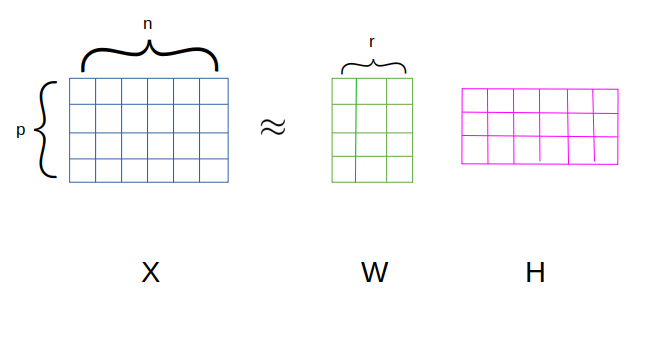
\includegraphics[scale=0.3]{../images/matrices.png}

%     \begin{itemize}
 %    \item $X \in R^{p \times n}$ : $X(:,j) = x_j$ for $1 \leq j \leq n$ %each column of the matrix $X \in R^{p x n}$ is a data point
  %   \item $W \in R^{p \times r}$ : $W(:,k) = w_k$ for $1 \leq k \leq r$ %each column of the matrix $W \in R^{p x r}$ is a basis element
   %  \item $H \in R^{r \times n}$ : $H(:,j) = h_j$ for $1 \leq j \leq n$ %each column of the matrix H gives the coordinates of a data point X(:,j) in the basis W
    % \end{itemize}

\end{frame}
